%%%%%%%%%%%%%%%%%%%%%%%%%%%%%%%%%%%%%%%%%%%%%%%%%%%%%%%%%%%%%%%%%%%%%%%%%%%%%%%%
%2345678901234567890123456789012345678901234567890123456789012345678901234567890
%        1         2         3         4         5         6         7         8

\documentclass[letterpaper, 10 pt, conference]{ieeeconf}  % Comment this line out if you need a4paper

%\documentclass[a4paper, 10pt, conference]{ieeeconf}      % Use this line for a4 paper

\IEEEoverridecommandlockouts                              % This command is only needed if 
                                                          % you want to use the \thanks command

\overrideIEEEmargins                                      % Needed to meet printer requirements.

\bibliographystyle{IEEEtran}

%In case you encounter the following error:
%Error 1010 The PDF file may be corrupt (unable to open PDF file) OR
%Error 1000 An error occurred while parsing a contents stream. Unable to analyze the PDF file.
%This is a known problem with pdfLaTeX conversion filter. The file cannot be opened with acrobat reader
%Please use one of the alternatives below to circumvent this error by uncommenting one or the other
%\pdfobjcompresslevel=0
%\pdfminorversion=4

% See the \addtolength command later in the file to balance the column lengths
% on the last page of the document

% The following packages can be found on http:\\www.ctan.org
\usepackage{graphicx} % for pdf, bitmapped graphics files
%\usepackage{epsfig} % for postscript graphics files
%\usepackage{mathptmx} % assumes new font selection scheme installed
%\usepackage{times} % assumes new font selection scheme installed
%\usepackage{amsmath} % assumes amsmath package installed
%\usepackage{amssymb}  % assumes amsmath package installed

\title{\LARGE \bf
Low-Pass Filtering for Accurate Measurement of Human Force Production During fMRI
}

\author{Ethan F. Oblak, Jarrod A. Lewis-Peacock, James S. Sulzer% <-this % stops a space
\thanks{This work is supported by a Robert J.\ Kleberg, Jr.\ and Helen C.\ Kleberg Foundation Medical Research Grant}%
\thanks{Ethan Oblak is with the Department of Mechanical Engineering, University of Texas at Austin, 78712, USA {\tt\small eoblak@utexas.edu}}%
\thanks{Jarrod Lewis-Peacock is with the Department of Psychology, University of Texas at Austin, 78712, USA {\tt\small jalewpea@utexas.edu}}%
\thanks{James Sulzer is with the Department of Mechanical Engineering, University of Texas at Austin, 78712, USA {\tt\small james.sulzer@utexas.edu}}%
}

\begin{document}

\maketitle
\thispagestyle{empty}
\pagestyle{empty}

%%%%%%%%%%%%%%%%%%%%%%%%%%%%%%%%%%%%%%%%%%%%%%%%%%%%%%%%%%%%%%%%%%%%%%%%%%%%%%%%
\begin{abstract}

This is the abstract.

\end{abstract}


%%%%%%%%%%%%%%%%%%%%%%%%%%%%%%%%%%%%%%%%%%%%%%%%%%%%%%%%%%%%%%%%%%%%%%%%%%%%%%%%
\section{INTRODUCTION}

Collecting measurements of human finger force production during fMRI scans can help explain how the brain produces fine motor skills \cite{wiestler2013skill, ejaz2015hand} and recovers after neurological injury such as stroke \cite{ejaz2018evidence}. Obtaining such recordings is difficult because of the strong static magnetic field of the MRI scanner and electromagnetic interference (EMI) experienced during fMRI echo-planar imaging (EPI). For safety, any force recording device must not incorporate any ferromagnetic components. Electronic components and wires are typically non-ferromagnetic and thus do not pose a major safety concern. However, the EMI during fMRI can corrupt force measurements from such devices. Although non-electronic sensors can be designed using fiber optics \cite{arata2013mri, butzer2015design}, such sensors suffer from drift, repeatability, and hysteresis issues \cite{han2017mri}.

Here, we characterize the effect of EMI on recordings from a piezoresistive force sensor similar to those used by other researchers \cite{diedrichsen2012two}. Although the use of these sensors has been reported in several fMRI studies \cite{diedrichsen2012two, wiestler2013skill, ejaz2015hand, ejaz2018evidence}, there are no details provided regarding the filtering necessary to achieve accurate force recordings. Therefore, we explored digital and analog filtering methods to reduce the effects of EMI on force recordings. Because human movement is inherently low-frequency ($<$20Hz), we specifically investigate low-pass filtering methods that preserve this signal. Finally, we provide overall recommendations for designing MRI-compatible devices with electronic force sensors, such as keyboards, grasp sensors, and robotics.

\section{MATERIALS AND METHODS}

\subsection{Force Sensitive Keyboard Design}

Our test fixture was an MRI-compatible 4-button response box (Fig.\ \ref{fig:setup}A) incorporating 4 piezoresistive force sensors with a force input range from 0-15N (FSS015WNGT; Sensing \& Control Honeywell Inc., Morristown, NJ). The differential output voltage signals from these sensors were transmitted to the MRI scanner control room via 50ft Cat5e Ethernet cables, which were also used to provide the excitation voltage for the sensors. Inside the control room, the force signals were amplified using an instrumentation amplifier (INA333; Texas Instruments, Dallas, TX), optionally filtered using a first-order RC low-pass filter, and digitally recorded using an Arduino device (Teensy 3.6; PJRC, Sherwood, OR). The force output from the sensors was truncated to 0-2N (typical of human finger pressing) and broadcast as 10-bit values from a USB human interface device (HID) using custom Arduino code, giving a resolution of 0.00195N/bit. Values were then recorded at 250Hz using Python and Pygame on a MacBook Pro.

% - Differential signal amplified by INA333 instrumentation amplifier: -0.03V to +0.3V range corresponds to 0-15N at input, output amplifier with 11k$\Omega$ resistor, $G = 1 + (100k\Omega \div R_g) = 10.09$; need 1.36N static force to register (3D printed key fixture ensures this), then have 4.505N/V resolution

% - Output of amplifier filtered by first-order RC low-pass filter: 2.2k$\Omega$ resistor and variable capacitor (to be tested)

% - Signal recorded by an Arduino (Teensy 3.6) at 250Hz with 13 bit resolution (0 to 3.3V), $2^{13} bits \div 3.3V = 2482 bits / V = 0.0004N = 0.05g$

% - output to computer: 0 to 5N at 10 bit resolution (joystick spoofing), 0.00488N/bit = 0.498g resolution

\subsection{fMRI Parameters}

Interference was generated using a Siemens Skyra 3T MRI scanner. A typical fMRI EPI sequence was tested (TR=2 sec; 26 slices; 3x3x3mm resolution; 64x64 matrix size; \textit{`singleband' or `SB' in figures and tables}) in addition to a higher resolution simultaneous multislice protocol (TR=2 sec; 40 slices; 2.3x2.3x2.3mm resolution; 100x100 matrix size; 2x multiband factor; \textit{`multiband' or `MB' in figures and tables}).

\subsection{Experimental Design}

A standard MRI phantom was placed inside a 32-channel head coil. The test fixture keyboard was placed at one of two positions inside the scanner: either (1) at the end of the scanner bore in the approximate position the keyboard would be placed if it were in the lap of a participant (\textit{`end' in figures and tables}) or (2) near the center of the scanner bore, touching the edge of the head coil (\textit{`center' in figures and tables}), as a worst-case scenario comparison (Fig.\ \ref{fig:setup}B,C). Baseline noise characteristics were evaluated with 5 minutes of non-scanning. Then, each of the 4 conditions (2 fMRI sequences x 2 keyboard positions) was testing with 5 minutes of fMRI EPI scanning.

% A 3Hz finger tapping task was recorded using a non-MRI-compatible reference force sensor and added to some of the noisy time series to determine how digital filtering affects task-based signals.

\begin{figure}[thpb]
  \centering
  \framebox{\parbox{3.25in}{
  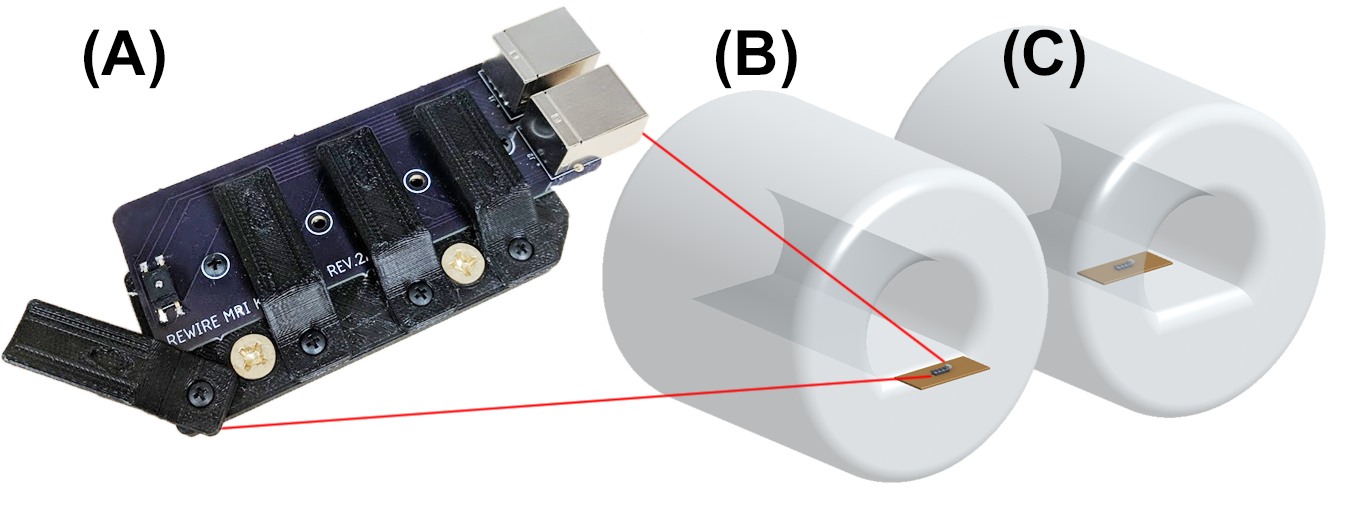
\includegraphics[width=3.25in,keepaspectratio]{fig-setup.png}
  }}
  \caption{\textbf{Experimental setup.} \textbf{(A)} 3D-printed keys applied a static force to each sensor (one key rotated to show the force transducer). The fixture was attached to a wooden board and placed either \textbf{(B)} at the end or \textbf{(C)} near the center of the MRI scanner bore.}
  \label{fig:setup}
\end{figure}

\subsection{Digital Filtering}

Real-time digital filtering was applied to the recorded signal using Python and SciPy (\texttt{scipy.signal.butter} and \texttt{scipy.signal.lfilter}). First-order Butterworth low-pass filters were implemented at 3 cutoff frequences: 10Hz, 30Hz, and 100Hz.

\subsection{Analog Filtering}

Post-amplifier analog filtering was achieved using RC filters ($C=0.5\mu F$) with cutoffs at 3 frequencies roughly matching the digital filters: 11.8Hz ($R=27k\Omega$), 31.8Hz ($R=10k\Omega$), and 96.5Hz ($R=3.3k\Omega$). Out of the 4 force recording channels, one was left unfiltered and each remaining channel used a different analog filter. \textit{For comparisons to digital filters, the nominal cutoff frequencies of 10Hz, 30Hz, and 100Hz will be used as labels for the analog filters.}

\section{FORCE RECORDINGS: MRI SCANNER IDLE}

We first investigated baseline noise characteristics of the force recordings, without running the MRI scanner. A summary of the results can be found in Table \ref{table:scanner-idle} and Fig.\ \ref{fig:scanner-idle}.

\begin{table}[h]
\caption{rms noise, scanner idle}
\label{table:scanner-idle}
\begin{center}
\begin{tabular}{|r||c|c|}
\hline
\textbf{Cutoff} & \textbf{Digital} & \textbf{Analog}\\
\hline
10Hz & 0.0020N & 0.0014N\\
\hline
30Hz & 0.0026N & 0.0015N\\
\hline
100Hz & 0.0034N & 0.0015N\\
\hline
None & 0.0036N & 0.0036N\\
\hline
\end{tabular}
\end{center}
\end{table}

\begin{figure}[thpb]
  \centering
  \framebox{\parbox{3.25in}{
  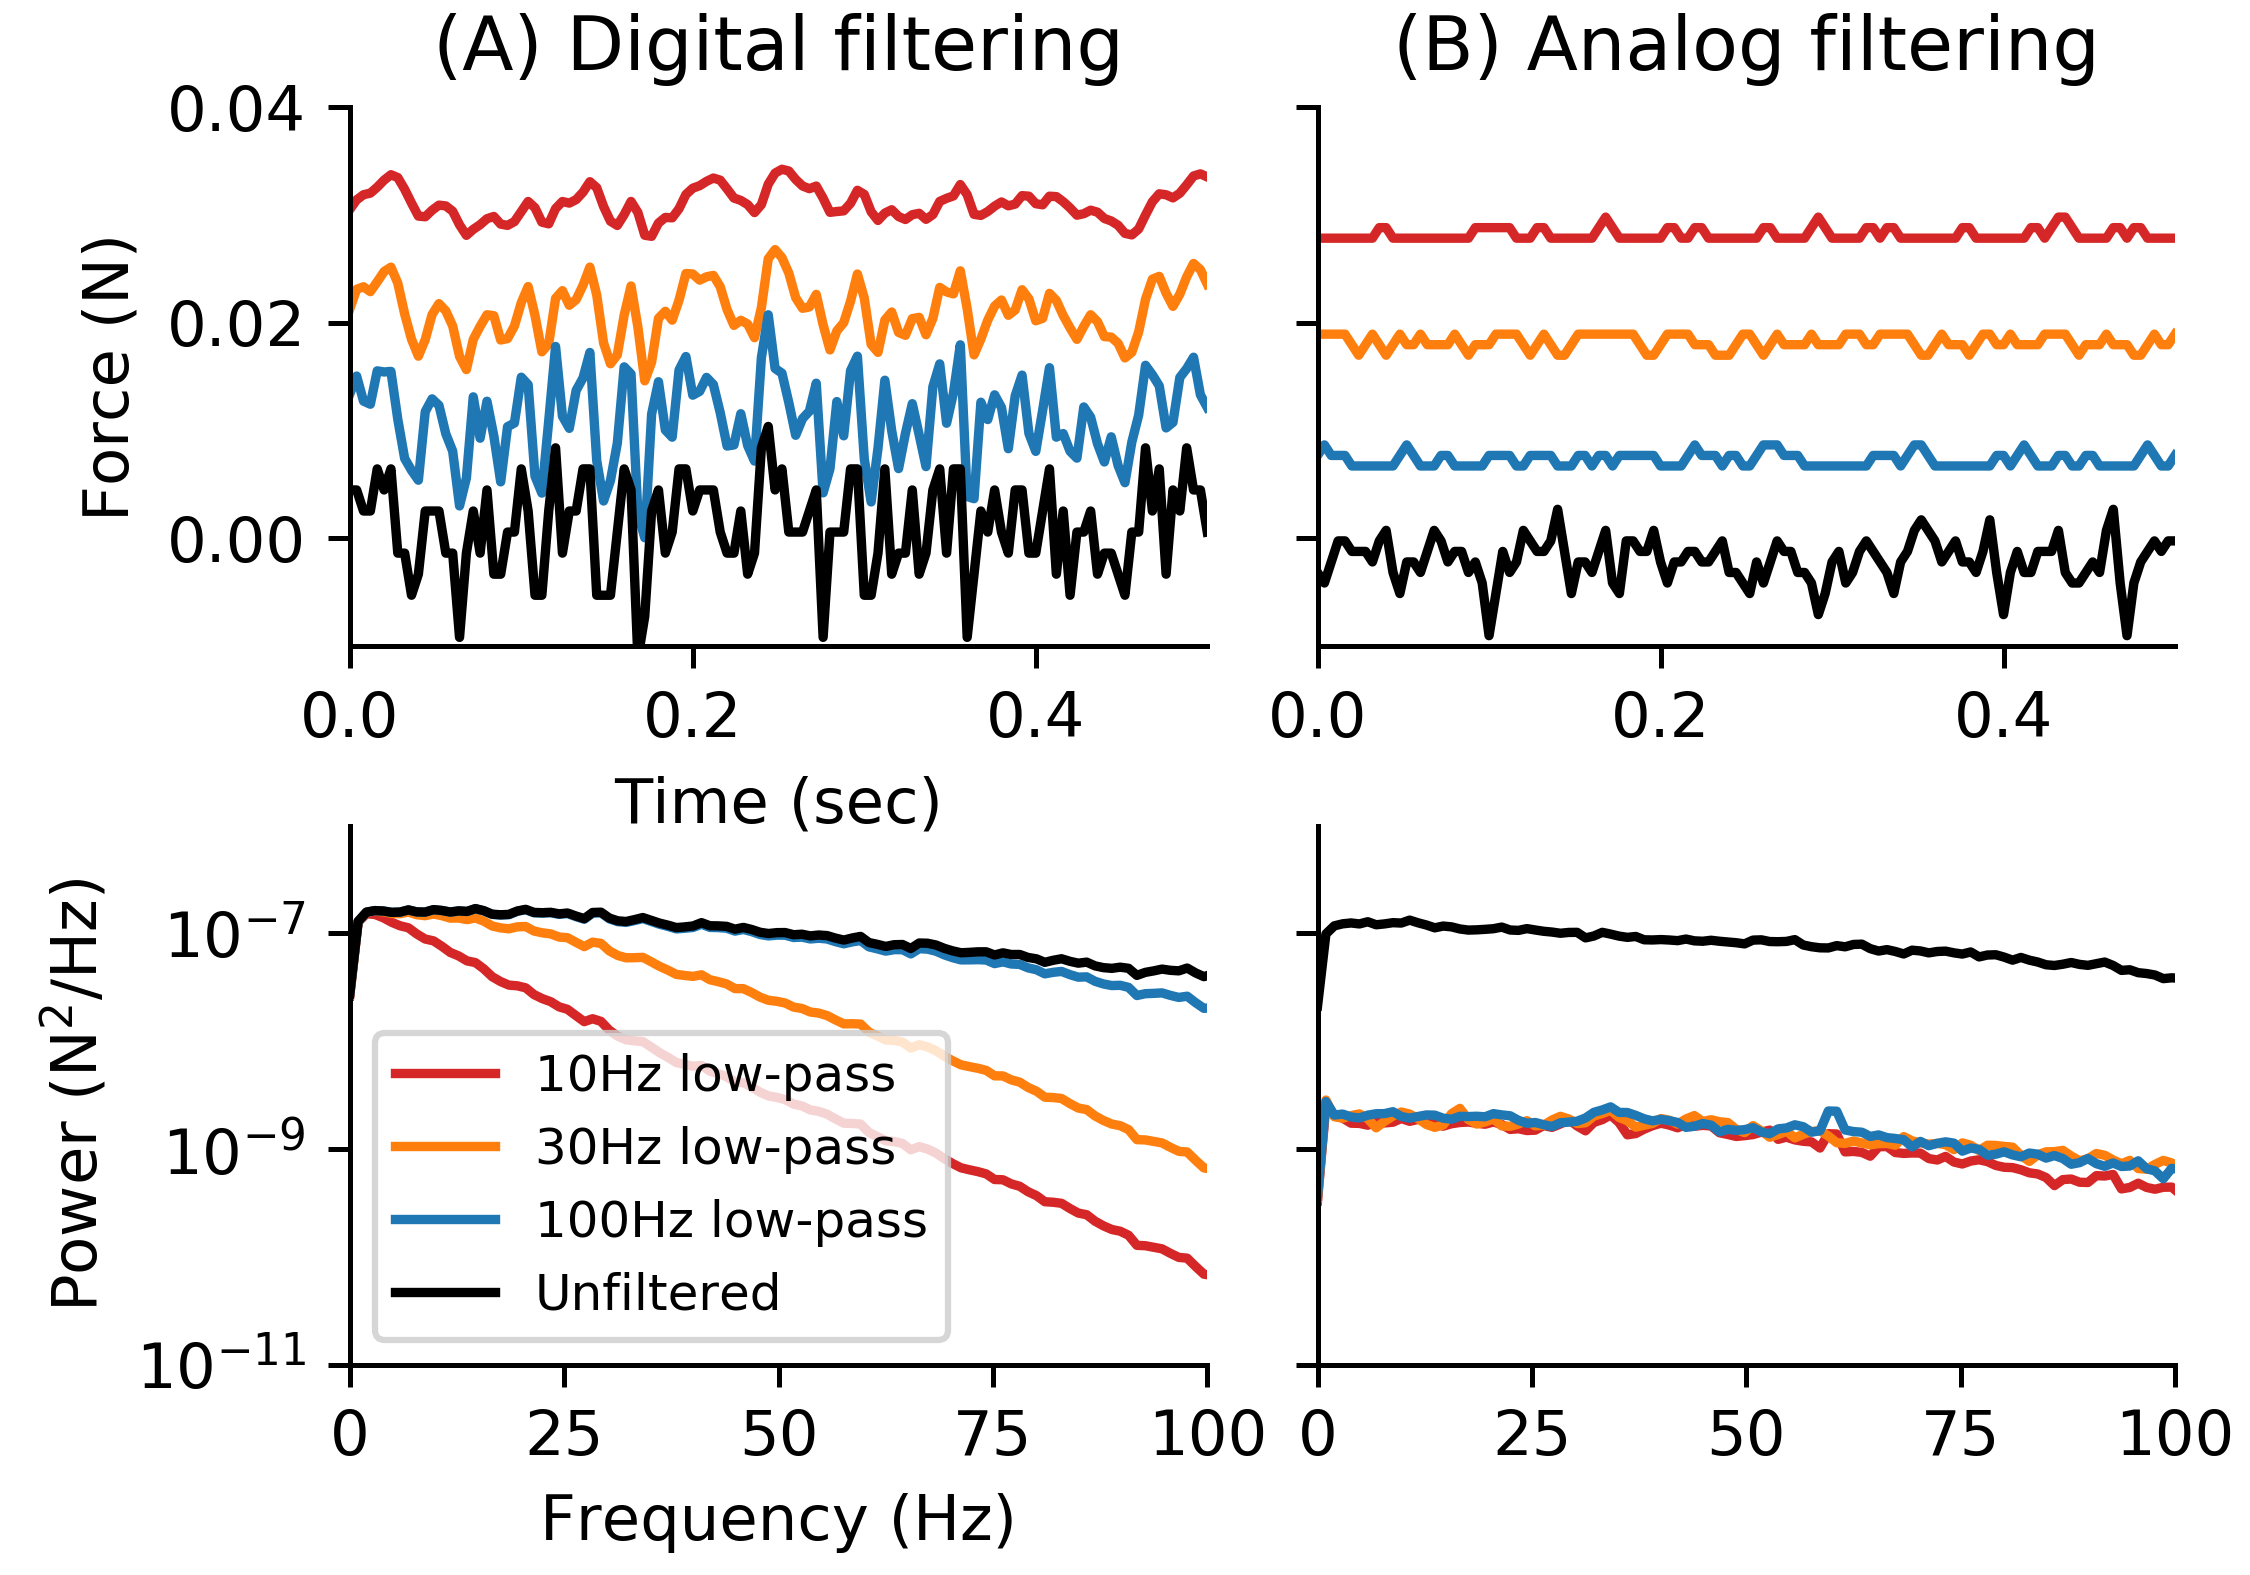
\includegraphics[width=3.25in,keepaspectratio]{fig-scanner-idle.png}
  }}
  \caption{\textbf{Time series and frequency response while MRI scanner idle.} \textbf{(A)} Digital filtering applied to baseline noise measurements. \textbf{(B)} Analog filtering applied to baseline noise measurements. Time series plots for each channel have been demeaned and are displayed at an offset for clarity.}
  \label{fig:scanner-idle}
\end{figure}

While both digital and analog filters reduce the baseline RMS noise, analog filtering is more effective because it acts as an anti-aliasing filter to reject broadband noise above the sampling frequency of 250Hz. All three analog filters reduce noise to negligible levels, below the analog to digital resolution of 0.00195N/bit, with a flat frequency spectrum (Fig.\ \ref{fig:scanner-idle}B, bottom), indicating that the source of noise must not originate from a frequency within that range of cutoffs (between 10Hz and 100Hz), but rather from a higher frequency. The time series of the analog filtered signals show a flat response with occasional discrete jumps (Fig.\ \ref{fig:scanner-idle}B, top) due to the limits of the analog to digital conversion. The digital filters, on the other hand, reduce noise as expected on the frequency spectrum, according to their cutoff frequencies (Fig.\ \ref{fig:scanner-idle}A, bottom). However, despite bringing RMS noise levels to similar levels as the analog filters, the digitally-filtered time series retain the shape of the unfiltered signal, albeit smoothed by the low-pass filtering (Fig.\ \ref{fig:scanner-idle}A, top).

\section{FORCE RECORDINGS: MRI SCANNER ACTIVE}

\subsection{Digital filtering}

We next investigated the effect of fMRI EPI on digitally-filtered force recordings. A summary of the results can be found in Table \ref{table:scanner-running-digital}, Fig. \ref{fig:scanner-running-digital}, and Fig. \ref{fig:scanner-running-digital-close}.

\begin{table}[h]
\caption{rms noise, scanner active, digital filtering}
\label{table:scanner-running-digital}
\begin{center}
\begin{tabular}{|r||c|c||c|c|}
\hline
\textbf{Cutoff} & \textbf{SB, end} & \textbf{MB, end} & \textbf{SB, center} & \textbf{MB, center}\\
\hline
10Hz & 0.0013N & 0.0014N & 0.0025N & 0.0029N\\
\hline
30Hz & 0.0021N & 0.0019N & 0.0040N & 0.0048N\\
\hline
100Hz & 0.0032N & 0.0031N & 0.0065N & 0.0075N\\
\hline
None & 0.0036N & 0.0036N & 0.0075N & 0.0082N\\
\hline

\end{tabular}
\end{center}
\end{table}

\begin{figure}[thpb]
  \centering
  \framebox{\parbox{3.25in}{
  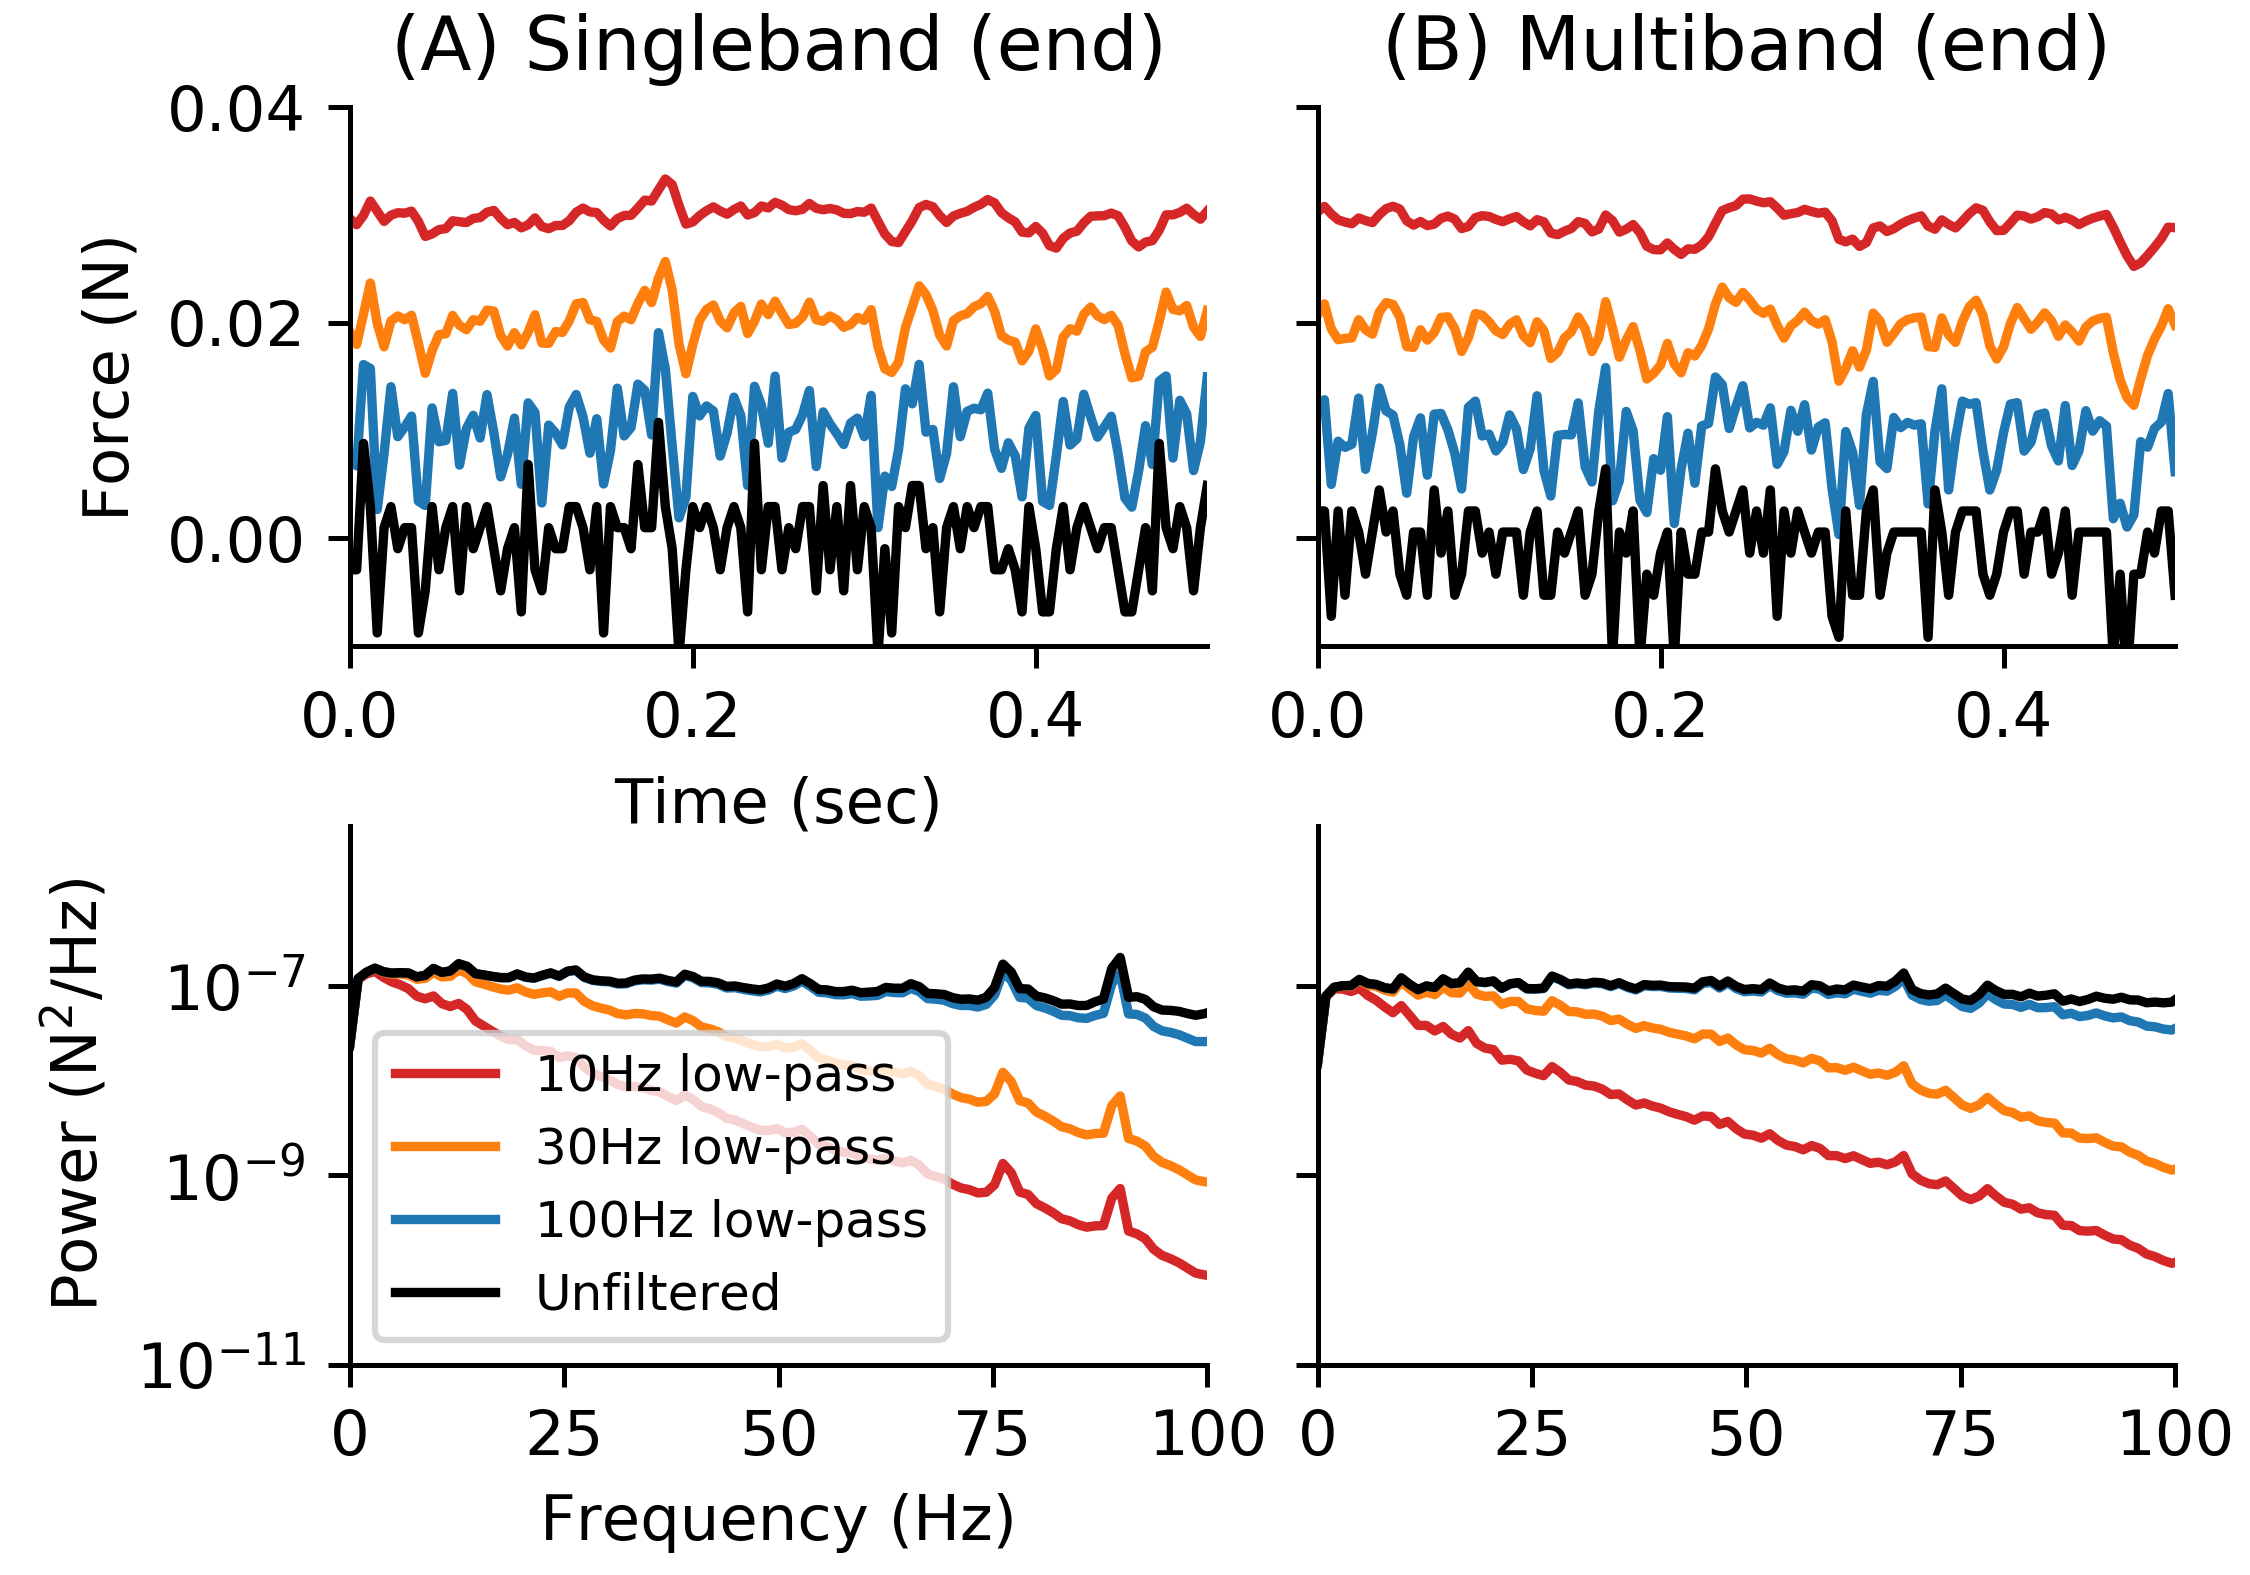
\includegraphics[width=3.25in,keepaspectratio]{fig-scanner-running-digital.png}
  }}
  \caption{\textbf{Effect of digital filtering on time series and frequency response during fMRI, keyboard at end of scanner bore.} \textbf{(A)} Digital filtering applied to baseline force recordings during standard fMRI. \textbf{(B)} Digital filtering applied to baseline force recordings during multiband fMRI.}
  \label{fig:scanner-running-digital}
\end{figure}

\begin{figure}[thpb]
  \centering
  \framebox{\parbox{3.25in}{
  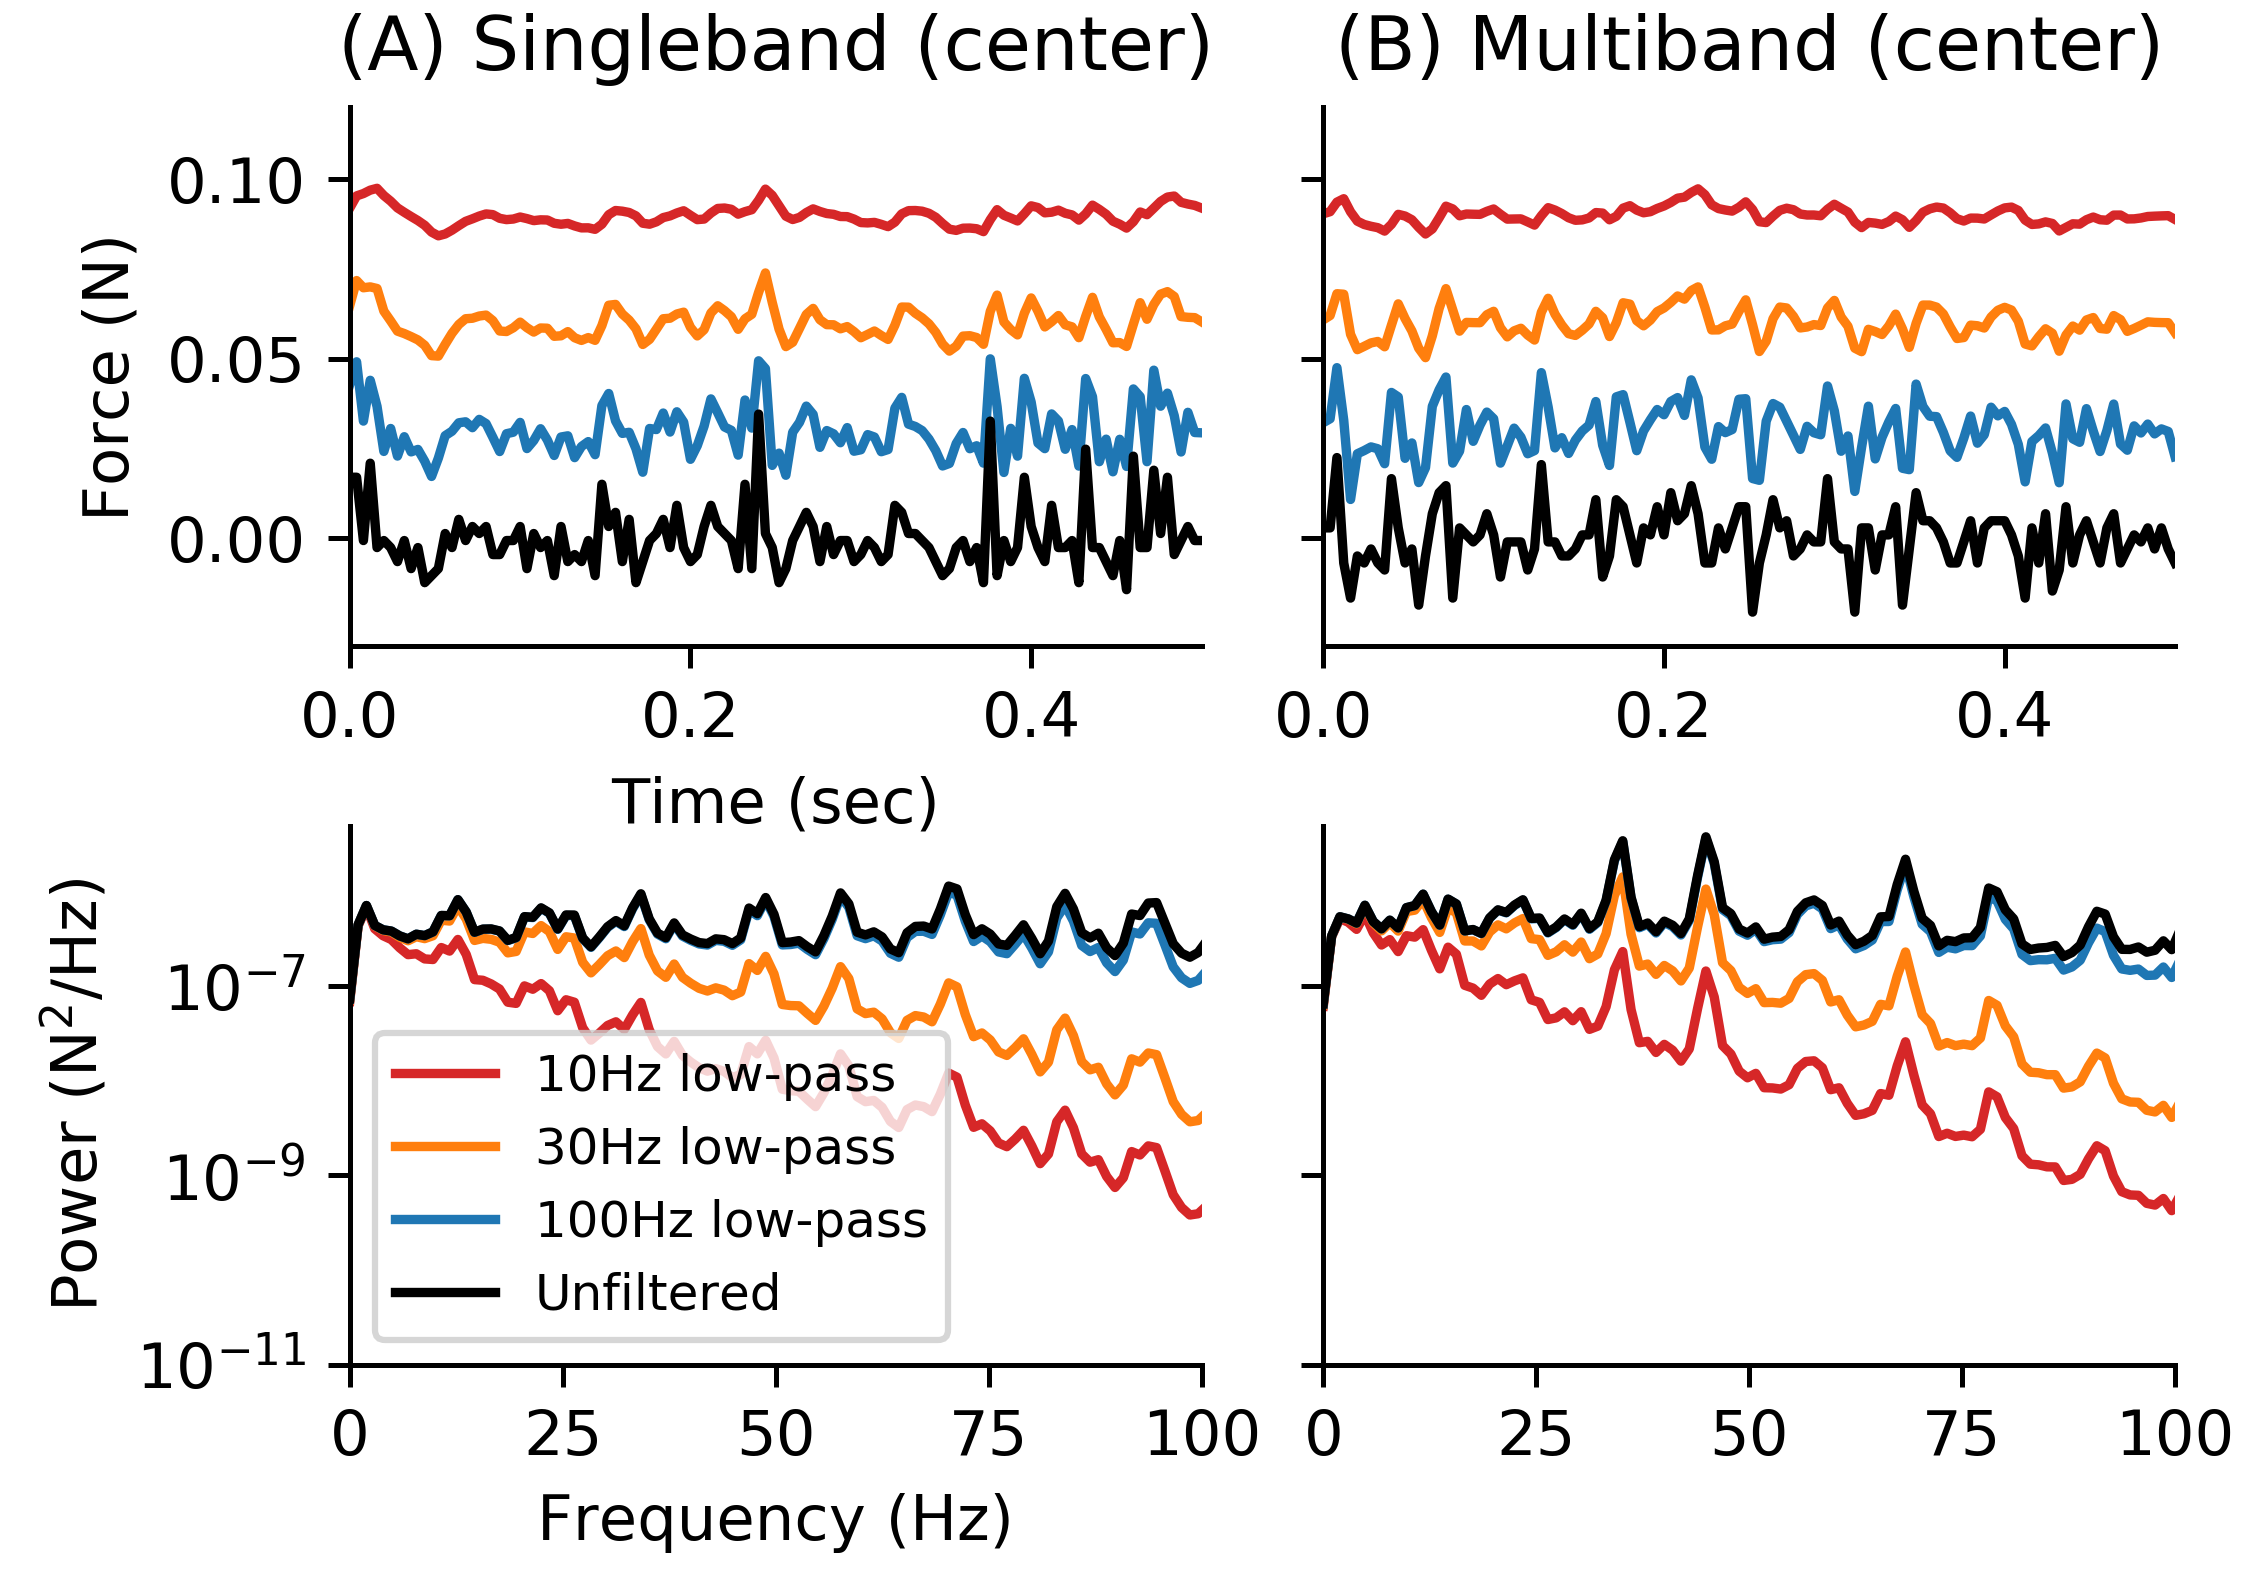
\includegraphics[width=3.25in,keepaspectratio]{fig-scanner-running-digital-close.png}
   }}
  \caption{\textbf{Effect of digital filtering on time series and frequency response during fMRI, keyboard near center of scanner bore.} \textbf{(A)} Digital filtering applied to baseline force recordings during standard fMRI. \textbf{(B)} Digital filtering applied to baseline force recordings during multiband fMRI.}
  \label{fig:scanner-running-digital-close}
\end{figure}

Both singleband and multiband protocols interfere with the force recordings. With the keyboard at the end of the bore, RMS noise levels are near the baseline level but interference can be seen in the frequency spectrum. At the center of the bore, RMS noise levels are approximately 2 times greater than at the end of the bore. At the end of the bore, digital low-pass filters are able to reduce RMS noise to similar levels as during baseline noise, although the time series retains the shape of the unfiltered signal (Fig.\ \ref{fig:scanner-running-digital}, top). The force recordings during fMRI show significant aliasing from high-frequency interference even at the end of the bore, as observed by the periodic shape of the frequency response (Fig.\ \ref{fig:scanner-running-digital}, bottom); this aliasing is even more pronounced at the center of the bore (Fig.\ \ref{fig:scanner-running-digital-close}, bottom). This interference pattern indicates that analog filtering will be necessary to properly filter out the noise introduced during fMRI.

\subsection{Analog filtering}

We then investigated the effect of fMRI EPI on force recordings when analog filters were used. A summary of the results can be found in Table \ref{table:scanner-running-analog}, Fig. \ref{fig:scanner-running-analog}, and Fig. \ref{fig:scanner-running-analog-close}.

\begin{table}[h]
\caption{rms noise, scanner active, analog filtering}
\label{table:scanner-running-analog}
\begin{center}
\begin{tabular}{|r||c|c||c|c|}
\hline
\textbf{Cutoff} & \textbf{SB, end} & \textbf{MB, end} & \textbf{SB, center} & \textbf{MB, center}\\
\hline
10Hz & 0.0017N & 0.0020N & 0.0246N & 0.1794N\\
\hline
30Hz & 0.0010N & 0.0010N & 0.0020N & 0.0056N\\
\hline
100Hz & 0.0018N & 0.0024N & 0.0054N & 0.0219N\\
\hline
None & 0.0036N & 0.0036N & 0.0075N & 0.0082N\\
\hline
\end{tabular}
\end{center}
\end{table}

\begin{figure}[thpb]
  \centering
  \framebox{\parbox{3.25in}{
  % 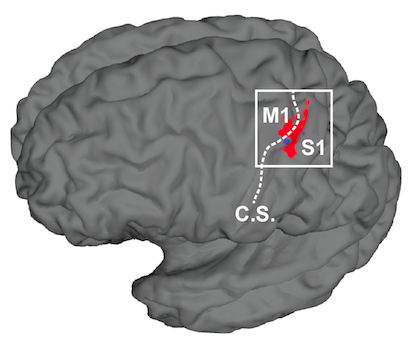
\includegraphics[width=3.25in,keepaspectratio]{test-brain.png}
  }}
  \caption{\textbf{Effect of analog filtering on time series and frequency response during fMRI, keyboard near end of scanner bore.} \textbf{(A)} Analog filtering applied to baseline force recording during standard fMRI. \textbf{(B)} Analog filtering applied to baseline force recordings during multiband fMRI.}
  \label{fig:scanner-running-analog}
\end{figure}

\begin{figure}[thpb]
  \centering
  \framebox{\parbox{3.25in}{
  % 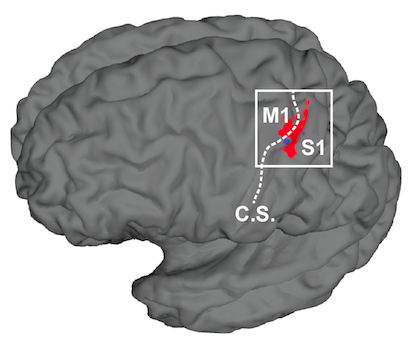
\includegraphics[width=3.25in,keepaspectratio]{test-brain.png}
  }}
  \caption{\textbf{Effect of analog filtering on time series and frequency response during fMRI, keyboard near center of scanner bore.} \textbf{(A)} Analog filtering applied to baseline force recording during standard fMRI. \textbf{(B)} Analog filtering applied to baseline force recordings during multiband fMRI.}
  \label{fig:scanner-running-analog-close}
\end{figure}

\subsection{Comparison of analog and digital filtering}

Finally, we can directly compare digital to analog filtering (Fig.\ \ref{fig:compare-digital-analog}).

\begin{figure}[thpb]
  \centering
  \framebox{\parbox{3.25in}{
  % 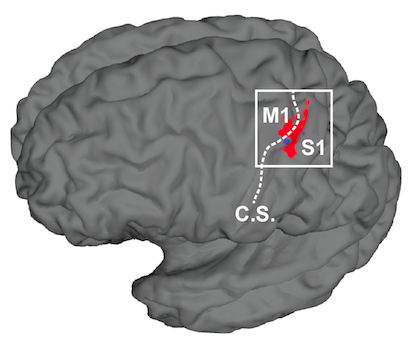
\includegraphics[width=3.25in,keepaspectratio]{test-brain.png}
  }}
  \caption{\textbf{Comparison of digital and analog filtering during fMRI.} \textbf{(A)} Comparison of 10Hz digital and analog low-pass filters during standard fMRI. \textbf{(B)} Comparison of 10Hz digital and analog low-pass filters during multiband fMRI.}
  \label{fig:compare-digital-analog}
\end{figure}

\section{RECOMMENDATIONS}

The ideal signal processing chain for accurate force measurements during fMRI includes an amplifier, a post-amplifier low-pass filter, and a high quality analog to digital conversion. For prototyping, it is possible to avoid using an amplifier and/or post-amplifier low-pass filter by using a digital low-pass filter, as long as the analog-to-digital conversion is at a high enough resolution and sampled at a high enough frequency to enable digital filtering. However, the artefacts introduced during fMRI are best handled using analog filtering because they occur at a much higher frequency than can easily be sampled. Even if the analog filters are above the Nyquist frequency of digital sampling, they are still able to reject a significant portion of the noise introduced by fMRI. Therefore, a conservative analog filter can be implemented in hardware, and additional digital filtering can be added in software, adjustable to the frequency of interest of the task given to human participants.

% \begin{figure}[thpb]
%   \centering
%   \framebox{\parbox{3.25in}{
%   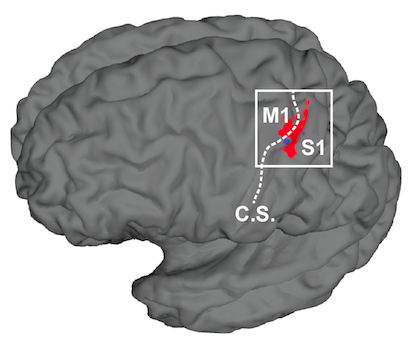
\includegraphics[width=3.25in,keepaspectratio]{test-brain.png}
%   }}
%   % 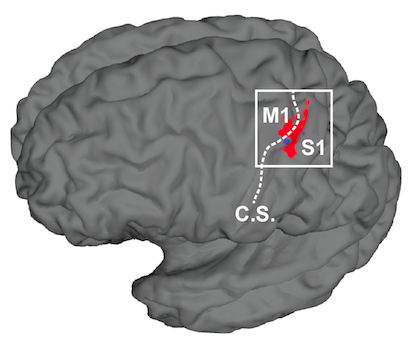
\includegraphics[scale=1.0]{test-brain.png}
%   \caption{Quisque interdum, velit et pellentesque sagittis, tortor elit congue diam, non facilisis nunc ligula sit amet turpis.}
%   \label{figurelabel}
% \end{figure}

\addtolength{\textheight}{-12cm}   % This command serves to balance the column lengths
                                  % on the last page of the document manually. It shortens
                                  % the textheight of the last page by a suitable amount.
                                  % This command does not take effect until the next page
                                  % so it should come on the page before the last. Make
                                  % sure that you do not shorten the textheight too much.

%%%%%%%%%%%%%%%%%%%%%%%%%%%%%%%%%%%%%%%%%%%%%%%%%%%%%%%%%%%%%%%%%%%%%%%%%%%%%%%%

\bibliography{references}


\end{document}
